\documentclass[fleqn]{jbook}
\usepackage{physpub}
% amsmath, graphicx は自動的に読み込まれるので
% \usepackage しないでください、してもかまわないけど。
\begin{document}

%%%%%%%%%%%%%%%%%%%%%%%% 問題 %%%%%%%%%%%%%%%%%%%%%%%%
\begin{question}{問題5}{林寛仁・太田良介}
図1に$\mathrm{NaI}$シンチレーションカウンター($\mathrm{NaI}$検出器)の原理的な構成を示す。この検出器はタリウムを混入したヨウ化ナトリウム$\mathrm{NaI(Tl)}$の結晶と光電子増倍管から出来ている。光電子増倍管の陽極から出力される電流パルスは抵抗
$\mathrm{R}=500 \ \mathrm{k\Omega}$と電気容量$\mathrm{C}=20 \ \mathrm{pF}$からなる等価回路で表される出力部回路に送られるものとする。この$\mathrm{NaI}$検出器を用いて、線源から放射されるガンマ線の検出を行う。以下の設問に答えよ。\\
 但し、光電子増倍管の陰極に光が入射してから増幅された電子群が陽極に達するまでの飛行時間は無視できるものとし、$\mathrm{NaI(Tl)}$結晶の蛍光減衰定数
$\mathrm{\tau}=230 \ \mathrm{ns}$とする。また、$\mathrm{NaI(Tl)}$結晶の寸法は、入射ガンマ線との相互作用で生じる2次ガンマ線の平均自由行程よりも小さいが、2次荷電粒子は$\mathrm{NaI(Tl)}$結晶内で完全に吸収される程度とする。
\begin{figure}[h]
  \begin{center}
    \resizebox{!}{30mm}{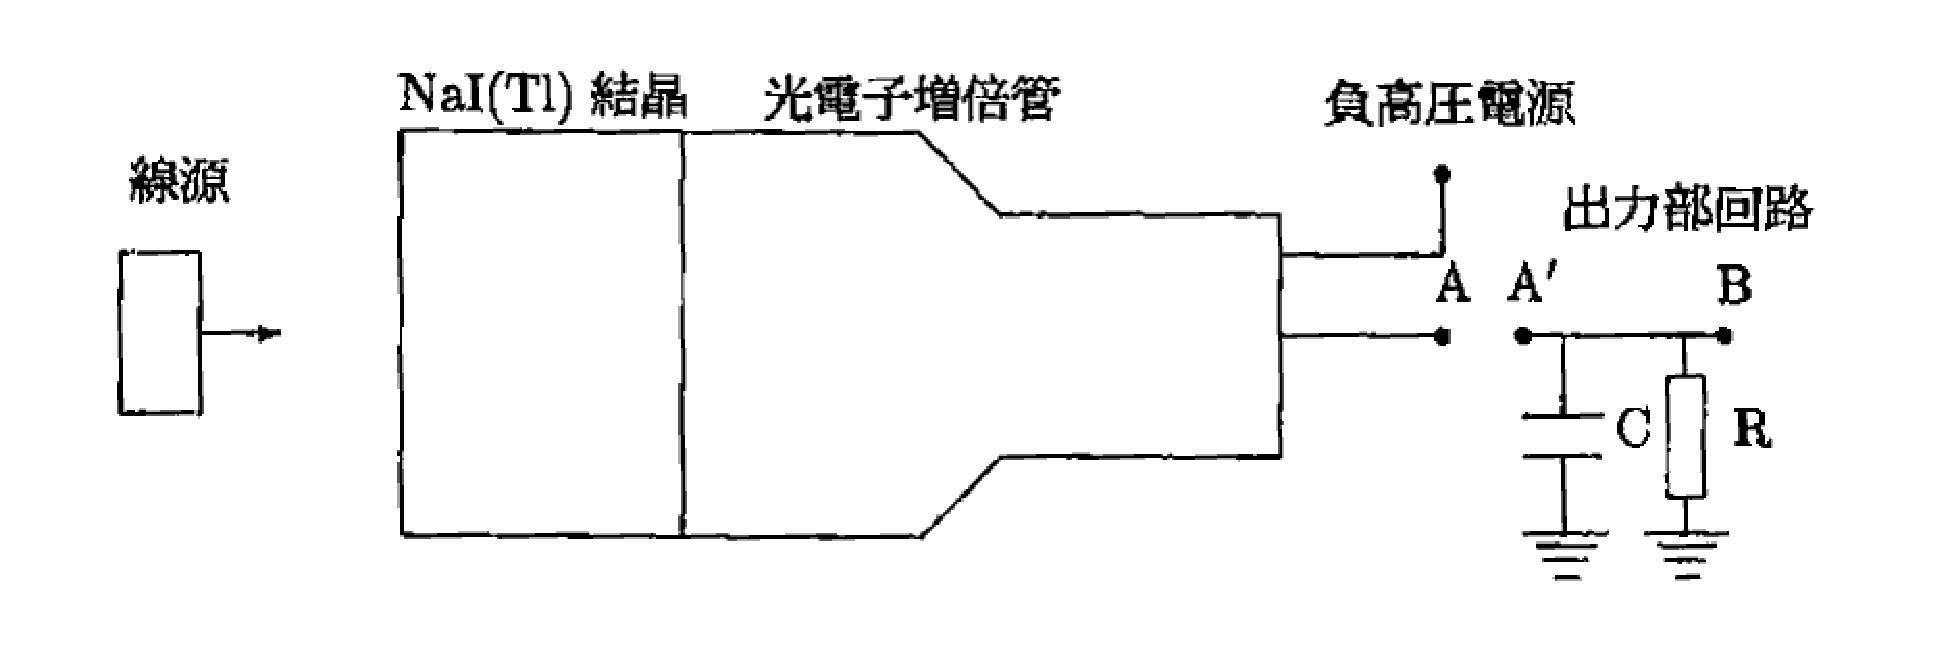
\includegraphics{2003phy5-1.eps}}
    \caption{$\mathrm{NaI(Tl)}$検出器の原理的な構成}
    \ilabel{NaIcounter}
  \end{center}
\end{figure}
\begin{enumerate}
\item ガンマ線が$\mathrm{NaI(Tl)}$の結晶中で起こす相互作用を3つ上げ、各々がどのような相互作用であるかを説明せよ。

\item 
\begin{enumerate}
	\item 図1で、点Aは光電子増倍管の陽極に同軸ケーブルでつながっているとする。点Aの出力をオシロスコープで見る場合、終端抵抗が必要であるが、その理由を述べ、接続の仕方を図示せよ。
	\item 電気的に正しく終端されたオシロスコープを用いて、点Aにおけるガンマ線から来る出力パルスはどのような波形に見えるかを図示せよ。また、点Aと点
	$\mathrm{A}^\prime$を結線して出力部回路をつないだ場合、点Bにおけるガンマ線からくるパルス波形を図示せよ。どちらの図に対しても、縦軸の電圧のスケールは任意でよいが、横軸の時間スケールが分かるように示すこと。
	\item 前問の点Bにおける波形観察の際、電気的なノイズが高く、ガンマ線からのパルス波形が見づらかったとする。その原因が特定されていない場合、どのような工夫を試みるべきか、具体的対処を2つあげよ。
\end{enumerate}

\item 出力部回路からの出力を適当な閾値によって波高弁別して計数した。線源をおかない場合、10分間で600カウントだった。線源をおいた場合、2分間で1000カウントだった。\begin{enumerate}
	\item 線源から放射されるガンマ線の計数率(カウント/分)とその標準偏差を求めよ。
	\item 線源から放射されるガンマ線の計数率を1%の精度で求めるには、合計何分間、線源を置いた計数を行えばよいか。但し、答えは分単位で小数点以下繰上げとする。また、線源をおかない計数をやり直さないとする。
\end{enumerate}

\item 線源から放射されるガンマ線のエネルギーが、(a)$0.5 \ \mathrm{MeV}$、(b)$5 \ \mathrm{MeV}$の単一エネルギーの場合において、出力部回路からのパルスをエネルギーに換算した度数分布を予想して図示せよ。その際、各々の分布の中で、設問1の相互作用がどの成分を占めるかもわかるように示すこと。

\item 設問4の(a)、(b)の2種類の線源から放射されるガンマ線のエネルギーがおおよそ分かっているが、正確には分かっていないとする。$\mathrm{NaI}$検出器を1個だけを用いても、バックグラウンド放射能が高いこと、および、設問1の3つの相互作用が混在することにより、エネルギーを正確に求めることが困難が状況とする。このような場合でも、同じ$\mathrm{NaI}$検出器を複数組み合わせる工夫によって、ガンマ線のエネルギーを正確に求められる。設問4の(a)、(b)各々の場合について、その工夫を図示し、ガンマ線のエネルギーが正確に求められる理由を説明せよ。
\end{enumerate}
\end{question}

%%%%%%%%%%%%%%%%%%%%%%%% 解答 %%%%%%%%%%%%%%%%%%%%%%%%
\begin{answer}{問題5}{林寛仁・太田良介}
\begin{enumerate}
\item 
\begin{itemize}
	\item 光電吸収\\
	光電吸収とは、入射ガンマ線光子が原子に束縛された電子と相互作用して全てのエネルギーを失い消失し、その電子が原子から飛び出す現象である。この場合入射光子エネルギー$h\nu$からもとの殻の電子の結合エネルギー$E_b$を差し引いた値の運動エネルギーを持つ光電子が吸収原子の電子殻の一つから作られる。光子が物質の原子によって吸収されるのは、原子の束縛電子によるものであって、自由電子による吸収は起こらない。運動量保存則よりこの過程で原子が反跳するが、反跳エネルギーは大変小さいので通常は無視できる。光電効果の起こる確率は、結合エネルギーが大きいほど、すなわち束縛電子と核との結びつきが強いほど大きい。これは、$h\nu$の光子の吸収では、電子の得る運動エネルギー$E$が、$E=h\nu - E_b$と表されることからも分かるように、$E_b$の大きい電子ほど飛び出す運動エネルギーが小さく、核に与える運動量が小さいからである。$K$電子の結合エネルギーより大きい場合は光電効果の80\%以上が$K$電子によるものとなり、また$K$電子の結合エネルギー以下では$K$電子による光電効果は起きない。他の殻についても同様であることから、各結合のエネルギーに相当する光子のところで吸収端を持つことになり、光電効果断面積は光子のエネルギーが小さくなるに従って不連続に増加する。一般的に光電効果断面積はシンチレーションカウンターの原子番号$Z$の$5$乗に比例して増大し、低エネルギーにおいては$(h\nu )^{-7/2}$,高エネルギーにおいては$(h\nu )^{-1}$に比例する。
	\item コンプトン散乱\\
	コンプトン散乱とは、入射ガンマ線光子が原子に束縛された電子と相互作用して反跳電子と散乱ガンマ線光子になる現象である。この場合散乱角に依存してこれら二つにエネルギーが分配される。
	\begin{figure}[h]
		\begin{center}
		\resizebox{!}{20mm}{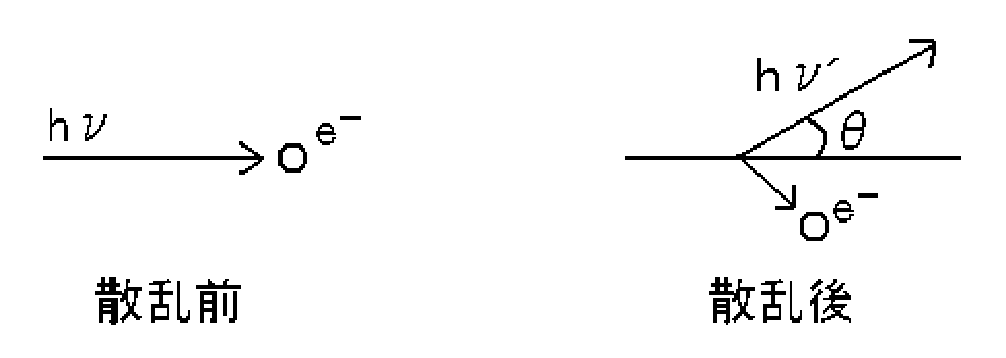
\includegraphics{2003phy5-2.eps}}
		\caption{コンプトン散乱}
		\ilabel{conpton}
  		\end{center}
	\end{figure}
光子のエネルギーが電子の結合エネルギーに比較して十分大きくなって電子を自由電子と見なすことが出来るなると、非弾性散乱を受ける。図\iref{conpton}の様に、散乱前は電子が静止していたと仮定して、散乱前の光子のエネルギーを$h\nu$、散乱光子のエネルギーを$h\nu^\prime$、電子の静止質量エネルギーを$m_0c^2$、散乱角を$\theta$とすると、エネルギーの関係は
	\begin{eqnarray}
		h\nu^\prime&=&\frac{h\nu}{1+\frac{h\nu}{m_0c^2}(1-\cos\theta)}\nonumber
	\end{eqnarray}
で表される。これより、コンプトン散乱によって得られる電子の運動エネルギー$E$は、
	\begin{equation}
		0 \le E \le \frac{2\frac{h\nu}{m_0 c^2}}{1+2\frac{h\nu}{m_0c^2}} 
		\cdot h\nu 										\nonumber
	\end{equation}
となり、連続的なエネルギー分布を取ることが分かる。これより、入射光子のエネルギーが非常に大きくなると、電子が得られる運動エネルギーは$E=h\nu - \frac{m_0 c^2}{2}\simeq h\nu - 0.26\ [\mathrm{MeV}]$に近づくことが分かる。また、コンプトン散乱断面積はシンチレーションカウンターの$Z$に比例する。しかし光電効果は1回だけ起こるものではなく複数回起こり得るので、このため、全エネルギーをシンチレーションカウンター内で電子に与えることになると、光電効果とほぼ同じエネルギーを与えることになるので、これにより光電効果と同等のイベントにもなりうる。また、これより、シンチレーションカウンターが大型になれば、コンプトン散乱が複数回行われる確率があがるため、光子の全エネルギーに相当する光電効果によるイベント数が見かけ上増えることになる。大型のシンチレーションカウンターでは光電効果よりもコンプトン散乱による全エネルギーに相当するイベントの割合が大きく、光電効果の断面積を用いて光電ピーク効率を計算することはできない。
	\item 電子対生成\\
	電子対生成とは、入射ガンマ線光子の完全な消滅位置に電子と陽電子の対を生成する現象で、$\mathrm{NaI}$の原子核中で陽子近傍の強い電場によって起こるものである。電子陽電子対を生成するには$2m_0c$のエネルギーが必要なので、この過程がエネルギー的に可能となるには$1.02 \ \mathrm{MeV}$以上のガンマ線エネルギーが必要である。$1.02 \ \mathrm{MeV}$を超えた分のガンマ線エネルギーは電子陽電子の運動エネルギーとなる。また、電子対生成断面積は$Z^2$に比例し、$\left(h\nu - 2m_0 c^2 \right)$に比例する。しかし、$Z$の大きい物質などの場合や高エネルギーの場合は$Z^2$はよい近似とはならない。対生成でできた電子、陽電子のうち、陽電子が対消滅により消滅すると2個の$0.51 \ \mathrm{MeV}$の光子を生ずるが、この光子は吸収される場合及びそのまま外に出る場合があり、二つとも吸収された場合はシンチレーションカウンター内で光子が消費したエネルギーが全て発光に寄与することになるので、これは、光電効果に含まれることになる。また、一つも吸収されない、または一つのみ吸収の場合のピークが、それぞれ光電ピークより$1.02 \ \mathrm{MeV}$、$0.51 \ \mathrm{MeV}$低いピークを作ることになるので、3つのピークが$0.51 \ \mathrm{MeV}$で並ぶことになる。この光子が吸収されずにコンプトン散乱を起こすことで連続的な分布を作ることになる。
\end{itemize}
\item 
\begin{enumerate}
	\item ケーブルの特性インピーダンスを$Z_0$としてケーブルの終端に抵抗$Z$を繋ぐと反射が起こり、その反射波の入射波に対する相対的波高$r$は
	\begin{equation}
		r=\frac{Z-Z_0}{Z+Z_0}							\nonumber
	\end{equation}
で表される。ここで、$Z_0$は、単位長さ当たりの抵抗であり、$Z$は同軸ケーブルの先に付ける抵抗値である。よって終端抵抗には$Z=Z_0$となるものを選ばなければ$r\ne 0$となるので反射波が存在し、OscilloScope上でその反射波も観測されることになり、正しい入射波を見ることが出来なくなる。よって、$Z=Z_0$とすることで、入射波のみを見ることが出来、繋ぎ方は図\iref{terminal}の様になる。一般的に$Z_0$は$50 \ \Omega$であり、終端抵抗として$Z= 50 \ \Omega$をとる。
	\begin{figure}[h]
  		\begin{center}
    	\resizebox{55mm}{!}{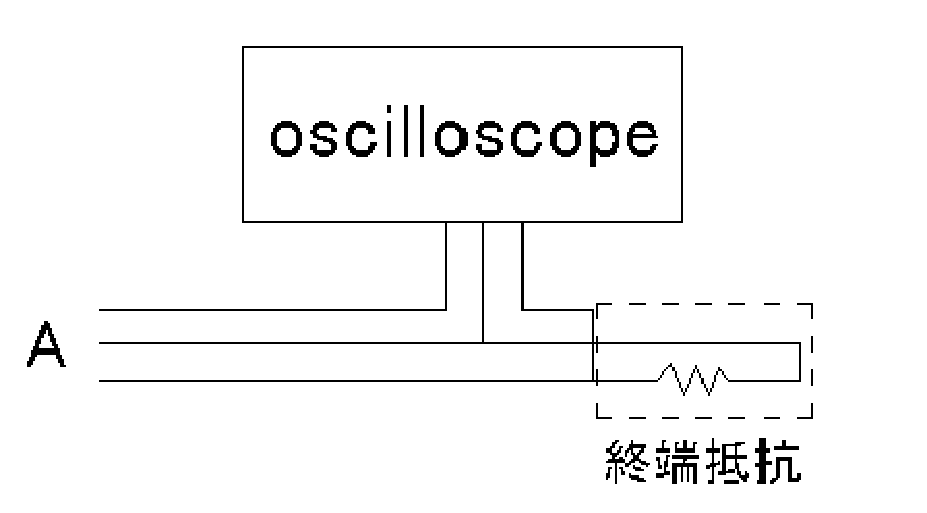
\includegraphics{2003phy5-3.eps}}
    	\caption{終端抵抗の繋ぎ方}
    	\ilabel{terminal}
  		\end{center}
	\end{figure}
	\item $\mathrm{NaI(Tl)}$結晶とガンマ線との相互作用で出来た高エネルギーの電子は、結晶内を通過することで他の電子を価電子帯から伝導体へ上げて数多くの電子正孔対を作る。このとき正孔はすばやく活性化物質の位置へ移動してそれを電離し、一方電子は結晶中を自由に移動して電離された活性化物質に出会うまで動く。そこで電子は活性化物質の位置に落ち込んで独自の励起エネルギー状態を持った中性の不純物配位を形成する。この状態から基底状態へある半減期(蛍光減衰定数)をもって遷移することで可視領域の光子が放出されるので、光子の放出量は指数関数的になる。この時電子の移動時間等は非常に短いので無視してよく、光電子増倍管からの出力パルスは光子の放出量に比例するので点Aにおいては$V_A(t)=V_0 e^{-\frac{t}{\tau}}$という形で表される。この場合$\tau =230 \ \mathrm{ns}$だから、その概形は図\iref{pulseA}の様になる。
	\begin{figure}[h]
  		\begin{center}
    	\resizebox{!}{40mm}{\includegraphics{2003phy5-4.eps}}
    	\caption{点Aにおける出力}
    	\ilabel{pulseA}
  		\end{center}
	\end{figure}
	次に点A、コンデンサ、抵抗に流れる電流をそれぞれ$I$、$I_1$、$I_2$とすると$I=I_1+I_2$が成り立つ。一方$I=I_0 e^{-\frac{t}{\tau}}$、$I_1=C\frac{\mathrm{d}V_B}{\mathrm{d}t}$、$I_2=\frac{V_B}{R}$だから、これらを代入して
\begin{equation}
	I_0 e^{-\frac{t}{\tau}}=C\frac{\mathrm{d}V_B}{\mathrm{d}t}
		+\frac{V_B}{R}								\nonumber
\end{equation}
この微分方程式を$V_B$について解く。まず左辺が0の場合の解は$V_B(t)=A e^{-\frac{t}{T}}$、但し$T=RC$、Aは時間によらない定数である。次に$A=A(t)$として上式に代入して計算すると、
\begin{eqnarray}
	\frac{\mathrm{d}A}{\mathrm{d}t}&=&\frac{RI_0}{T}
		e^{\left(\frac{t}{T}-\frac{t}{\tau}\right)}	\nonumber\\
	\therefore \ \ A(t)&=&RI_0\frac{\tau}{\tau -T}
		e^{\left(\frac{t}{T}-\frac{t}{\tau}\right)}	\nonumber
\end{eqnarray}
よって
\begin{equation}
	V_B=RI_0\frac{\tau}{\tau -T}
		e^{-\frac{t}{\tau}}
		+Ae^{-\frac{t}{T}}							\nonumber
\end{equation}
初期条件は$t=0$の時$V_B=0$だから、$A=-RI_0\frac{\tau}{\tau -T}$、結局
\begin{equation}
	V_B=RI_0\frac{\tau}{\tau -T}\left(
		e^{-\frac{t}{\tau}}
		-e^{-\frac{t}{T}}\right)					\nonumber
\end{equation}
となる。$T=10\mathrm{\mu s}$だから、その概形は図\iref{pulseB}の様になる。
	\begin{figure}[h]
  		\begin{center}
    	\resizebox{!}{40mm}{\includegraphics{2003phy5-5.eps}}
    	\caption{点Bにおける出力}
    	\ilabel{pulseB}
  		\end{center}
	\end{figure}
	\item 
Discriminatorのスレッショルドを用いて低いノイズをカットしたり、出力の先にハイパスフィルターやローパスフィルターを付けてノイズを落としたり、出力を増幅させてS/N比を改善したりする。他にも、PMTのゲインが安定していないことも考えられる。これを解決するには、まず、同程度のRateを長い時間NaI(Tl)検出器に入射させ続けることで慣らす。また、印加電圧が高いとゲインが印加電圧やPMTの中のダイノードの段数に大きく依存するために、例えばMicrochannel\ Plate等なるべく低い段数のものを用いたり、印加電圧をできるだけ低くて済むようにしたりする。印加電圧が高いとゲインが一定にならないだけでなく、ノイズも増やしてしまう可能性もあるため、あまりよくない。

\end{enumerate}
\item 
\begin{enumerate}
	\item 一事象当たりの確率は同じ状況で測定し、計数時間が放射線の半減期に比べて短いことを仮定すれば一定であり、かつその確率は低い。また、試料中の原子核の総数が大きい。これより、反応が起こる確率$p$が小さく、試行回数$n$大きい場合は、2項分布で起きる確率$P(x)$は$\frac{n!}{(n-x)!} \simeq n^x$,$(1-p)^{n-x} \simeq \mathrm{e} ^{-pn}$を用いて、以下のようにポアソン分布の近似に近似できることになる。
\begin{eqnarray}
	P(x) &=& \frac{n!}{(n-x)!x!}p^x(1-p)^{n-x}				\nonumber \\
		&\simeq& \frac{\left(pn\right)^x \mathrm{e} ^{-pn} }{x!} \nonumber \\
		&=& \frac{\left(\overline{x}\right)^x \mathrm{e} ^{-\overline{x}}}{x!}
		\nonumber
\end{eqnarray}
ここで、$\overline{x}$は分布の平均値であり、$\overline{x} = pn$である。これより、ポアソン分布の近似が十分に成立しているものと仮定できるので、よって、ガンマ線のカウント数をmとしたとき、その標準偏差は以下のように求められる。
\begin{eqnarray}
	\sigma ^2 &=& \sum_{x=0}^{n} (x- \overline{x})^2 \cdot P(x) 
		= pn								
		= \overline{x}					\nonumber \\
	\sigma &=& \sqrt{\overline{x}}			\nonumber
\end{eqnarray}
よって、$\sigma=\sqrt{m}$で与えられる。線源をおかない場合の計数率は$m_1=600[/10\mathrm{min}]=60[/\mathrm{min}]$、標準偏差は$\sigma_1=\sqrt{m_1}\simeq 24[/10\mathrm{min}]=2.4[/\mathrm{min}]$となる。次に線源をおいた場合を考えると、全体の計数率は$m=1000[/2\mathrm{min}]=500[/\mathrm{min}]$、標準偏差は$\sigma=\sqrt{m}\simeq 32[/2\mathrm{min}]=16[/\mathrm{min}]$となる。よって線源から放射されっるガンマ線の計数率は$m_2=m-m_1=440[/\mathrm{min}]$、誤差伝播より$\sigma_2=\sqrt{\sigma^2+{\sigma_1}^2}\simeq 16[/\mathrm{min}]$となる。
	\item 必要なカウント数を$N$、要する時間を$m[\mathrm{min}]$とすると全体の計数率と標準偏差は
\begin{equation}
n_{tot}=\frac{N}{m} \ [\mathrm{min}^{-1}] \ , \ 
\sigma_{tot}=\frac{N}{\sqrt{m}} \ [\mathrm{min}^{-1}]
\end{equation}
よって線源については
\begin{equation}
n_s=\frac{N}{m}-n_1=\frac{N}{m}-60 \ [\mathrm{min}^{-1}] \ , \ 
\sigma_s=\sqrt{\sigma_{tot}^2+\sigma_1^2}
=\sqrt{\frac{N}{m^2}+6} \ [\mathrm{min}^{-1}]  
\end{equation}
(i)より$N\simeq 500m$なので
\begin{equation}
n_s=440 \ [\mathrm{min}^{-1}] \ , \ \sigma_s=
\sqrt{\frac{500}{m}+6} \ [\mathrm{min}^{-1}]
\end{equation}
精度を1%とするには
\begin{equation}
\frac{\sigma_s}{n_s}=\frac{1}{10^2} \ \ \ \ \therefore
m\simeq 37.4 \ [\mathrm{min}]
\end{equation}
なので、時間は$38$分必要である。
\end{enumerate}

\item 

(a)$0.5 \ \mathrm{MeV}$のとき\\

\begin{figure}[h]
		\begin{center}
		\resizebox{!}{90mm}{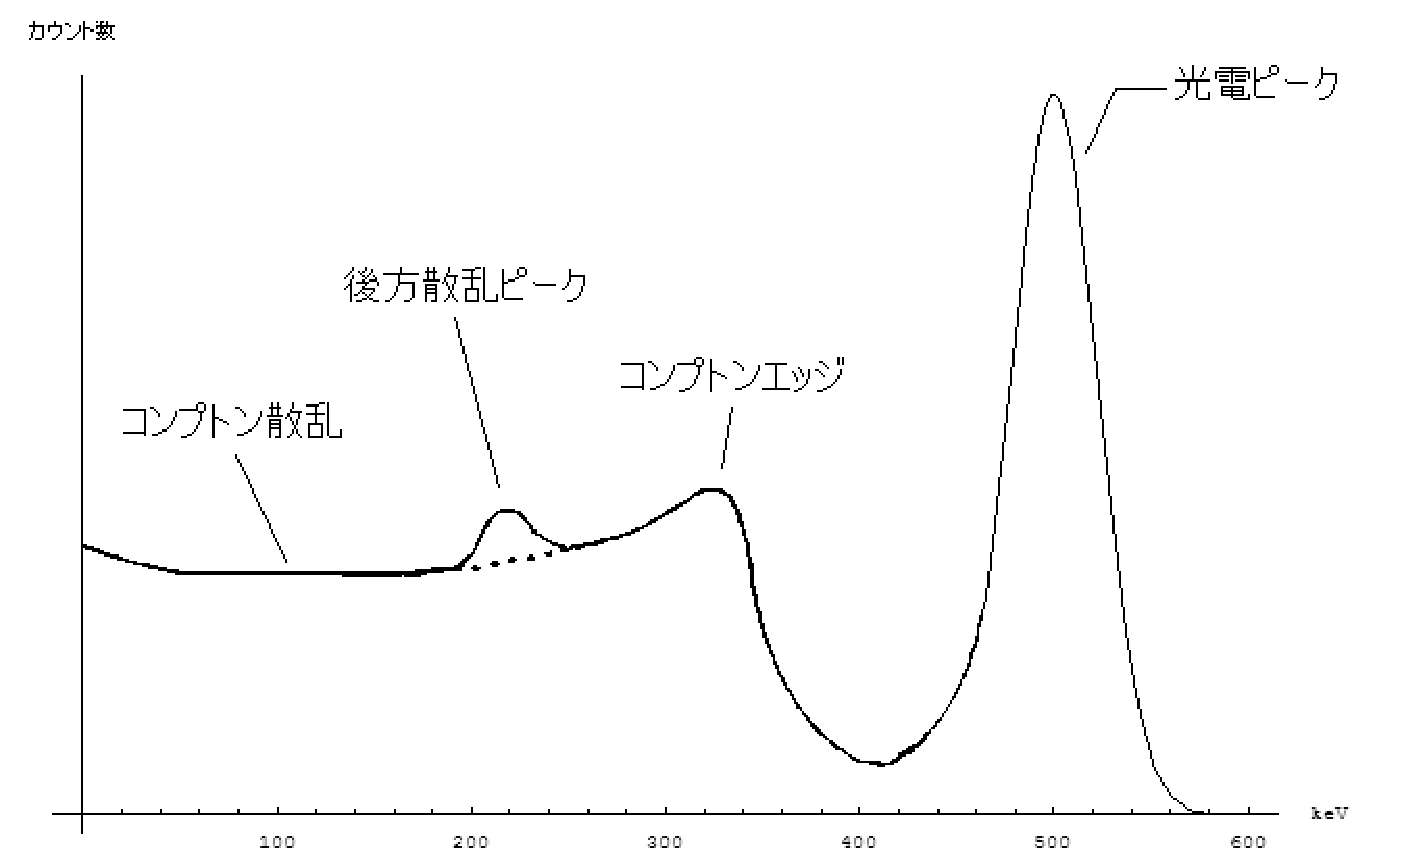
\includegraphics{2003phy5-6.eps}}
		\caption{$0.5 \ \mathrm{MeV}$における度数分布}
		\ilabel{500KeVenergy}
  		\end{center}
\end{figure}

$0.5 \ \mathrm{MeV}$におけるガンマ線のNaI(Tl)シンチレーターにおける断面積は
\begin{eqnarray}
	コンプトン散乱>光電効果\gg 0=電子対生成	\nonumber
\end{eqnarray}
であるので、これよりグラフは以下のようになる。

ここで、後方散乱ピークがない理想的な場合は、そこの部分が点線で示してある。電子対生成によるピークは電子静止質量の2倍のエネルギーよりも小さいので起こらず、全エネルギーピークはこの場合は問題の設定から大半は光電効果によるものである。\\
\\
(b)$5 \ \mathrm{MeV}$のとき\\

\begin{figure}[h]
		\begin{center}
		\resizebox{!}{90mm}{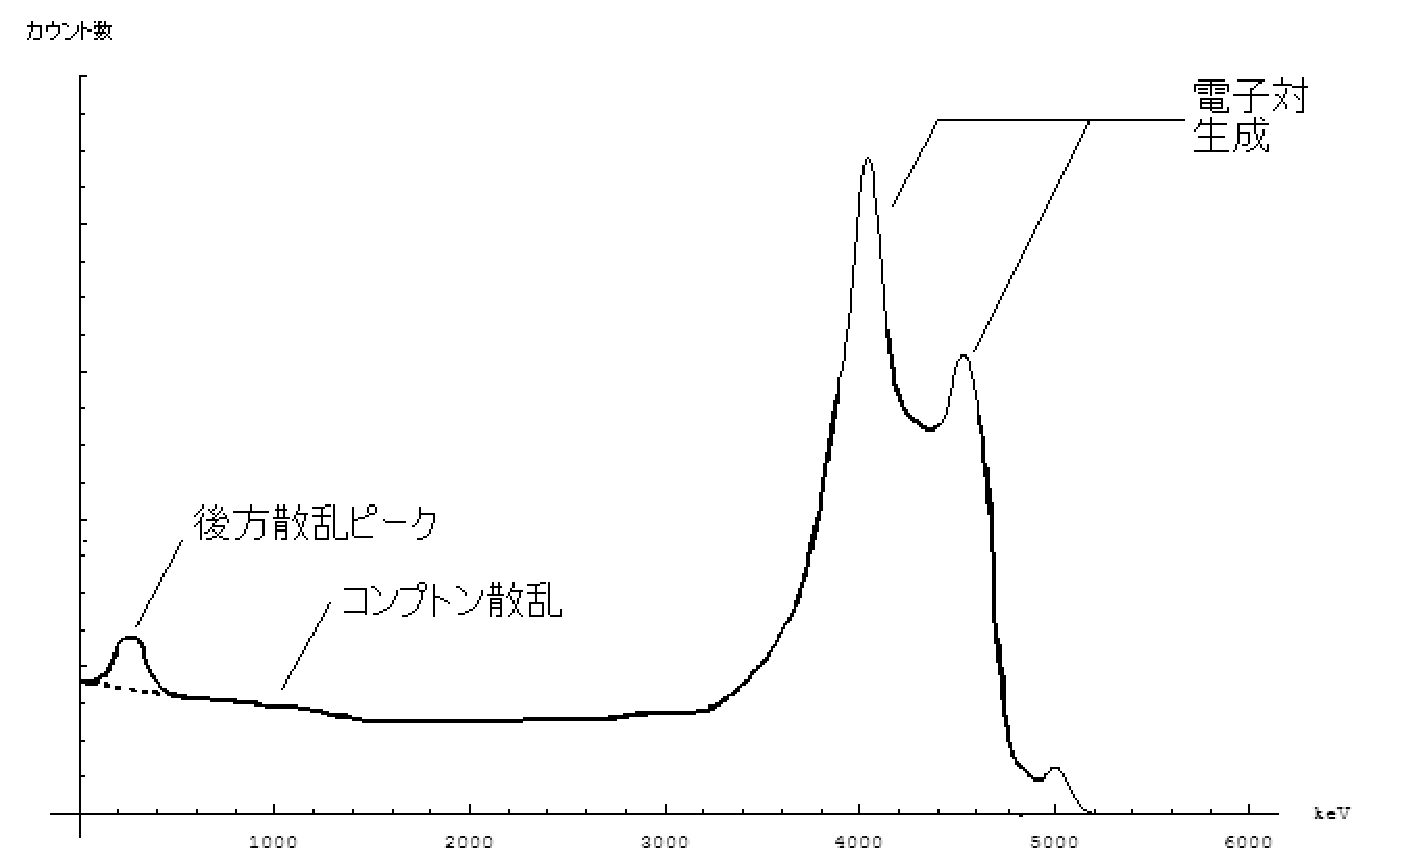
\includegraphics{2003phy5-7.eps}}
		\caption{$5 \ \mathrm{MeV}$における度数分布}
		\ilabel{5MeVenergy}
  		\end{center}
\end{figure}

この場合は入射ガンマ線のエネルギーが大きいために断面積が、
\begin{eqnarray}
	コンプトン散乱>電子対生成 \gg 光電効果\simeq 0		\nonumber
\end{eqnarray}
となり、また、NaI(Tl)結晶の寸法は、入射ガンマ線との相互作用で生じる2次ガンマ線の平均自由行程よりも小さいが、2次荷電粒子はNaI(Tl)結晶内で完全に吸収される程度という問題の設定から、コンプトン散乱及び電子対生成による全エネルギーピークはほとんど得られず、光電効果はほとんど起こらないので、全エネルギーピークはほとんど無くなる。うちわけのほとんどは、コンプトン散乱したものが光電効果によって全エネルギーを落としたり、電子対生成したあとの、陽電子による電子との対消滅による2本の$511 \ \mathrm{keV}$のガンマ線が光電効果を起こすなどの、複数の効果の組み合わせによるため、一意に(a)のときのように光電効果によるピークとは決めることが出来ない。また、度数分布は以下のようになり、ここでも(a)と同様に後方散乱ピークがない理想的な場合は、点線で示してある。電子対生成によるピークが2本見えるのは、陽電子が電子と対消滅したときに出来るガンマ線が0本、1本、2本検出器内にエネルギーを落とすことがあるからであり、この問題設定では、NaI(Tl)結晶の大きさがさほど大きくないことから、2本とも全エネルギーを落とす確率は小さいので、全エネルギーより$511 \ \mathrm{keV}$及び$1022 \ \mathrm{keV}$小さい2つのピークが主に見えるためである。グラフの形状は、NaI(Tl)結晶の大きさに依存し、大きくすればするほど相対的に全エネルギーピークが増え、その他のピークが減ることになる。問題の設定よりNaI(Tl)結晶の大きさは、6割の確率で2次ガンマ線が相互作用すると仮定してグラフは作った。

\item 

(a)$0.5 \ \mathrm{MeV}$のとき\\

\begin{figure}[h]
		\begin{center}
		\resizebox{!}{100mm}{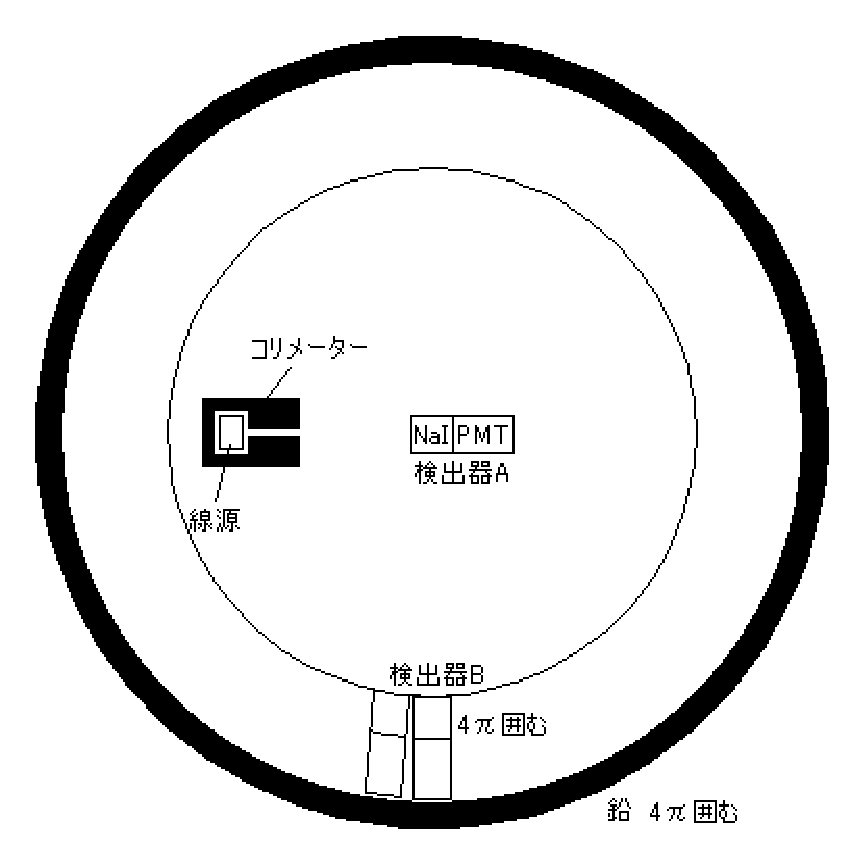
\includegraphics{2003phy5-8.eps}}
		\caption{(a)の実験装置の配置}
		\ilabel{0.5MeV setup}
  		\end{center}
\end{figure}

$0.5 \ \mathrm{MeV}$におけるガンマ線のNaI(Tl)シンチレーターにおける断面積は\\
\begin{eqnarray}
	コンプトン散乱>光電効果\gg 0=電子対生成	\nonumber
\end{eqnarray}
であり、コンプトン散乱と光電効果の断面積のオーダーはほぼ同じであるので、このことから、実験装置としては、コリメーター等を用いてまずガンマ線源から出てきたガンマ線が全て検出器に入るようにする。便宜上この検出器を検出器Aと呼ぶことにする。このまま測定すれば、結果は上記の断面積のとおりに前問のグラフで書けとあったようになり、連続的なコンプトンピーク及びコンプトンエッジと全エネルギーピークである光電ピークとバックグラウンドが主に見えることにるので、、まず、検出器とガンマ線源を大量の検出器で4$\pi$覆う。理想的にはNaI(Tl)よりもBGO等を使いった方がよいのだが問題の設定上NaI(Tl)を用いることとする。そして、外側の覆っている全ての検出器を便宜上検出器Bと呼ぶことにする。ここで、$A∩\overline{B}$という逆計数測定を行う。すると、検出器Bを鳴らしたものはカウントされなくなるので、検出されるイベントがどのようなものがあるかを検討すると、
\begin{enumerate}
\item
光電効果\\
入射ガンマ線は全エネルギーを検出器Aで失っており、全エネルギーピークを形成し、また検出器Bは鳴らさないので、カウントされる。
\item
コンプトン散乱\\
1回のコンプトン散乱によりガンマ線が失うエネルギーは運動量保存則及びエネルギー保存則からすぐ計算できるように全てではなく、全エネルギーを失わない。これにより、ガンマ線が検出器Aの外に逃げるものがある。もちろんコンプトン散乱は1回ではなく、複数起こる可能性もあり、また光電効果等も起こる可能性があるので、全エネルギーを失う可能性もある。これは検出器が大きくなると、光電ピークと呼ばれる全エネルギーピークが増えることに該当する。これより、検出器Aで全エネルギーを失わなかったイベントは検出器Bも鳴らすことになるので、このイベントは落ちる。当然全エネルギーを検出器Aで失えば検出器Bは鳴らないので、このイベントはカウントされることになる。
\item
電子対生成\\
この場合は入射エネルギーが電子の2倍の質量よりも小さいので起こらないが、仮に起こった場合でも、生成された電子と陽電子はすぐにとまり、ここで陽電子は電子と対消滅して、2本の$511 \ \mathrm{keV}$のガンマ線を作るが、この2本のガンマ線もコンプトン散乱で議論したのと同様に、検出器Aで全エネルギーを失わなければ検出器Bをならすことに鳴るので、カウントされなくなり、結局全エネルギーを落とした場合のみのイベントが残ることになる。
\item
バックグラウンド\\
バックグラウンドは、覆われている中のところで発生して、それが検出器Aにおいて全エネルギーを落とすという、ほとんど考えられないケースを除くと、必ず検出器Bも鳴ることになるので、これより、バックグラウンドによるイベントも落ちることになる。
\end{enumerate}
以上から、全エネルギーピークのみが残ることになる。これは、NaI(Tl)結晶の寸法は、入射ガンマ線との相互作用で生じる2次ガンマ線の平均自由行程よりも小さいが、2次荷電粒子はNaI(Tl)結晶内で完全に吸収される程度という問題の設定から、おそらくほぼ全ての全エネルギーピークは光電ピークからなると考えられる。これより、バックグラウンドを排除して、さらに全エネルギーのピークのみを取り出すことが可能となる。また、さらに検出器全体を鉛で覆うと、よりバックグラウンドを除くことが出来る。これにより、環境放射線のガンマ線や、アルファ線は鉛の厚さを数cm程度にしておくことで鉛中で止まり、検出器内に入らないで済み、二次宇宙線がバックグラウンドとして残ることになる。二次宇宙線は高エネルギーの$\mu$粒子が主で、残りが電子であり、その運動エネルギーのオーダーはGeVであるので、これを鉛で止めるためには、最小電離損失が$-\frac{ \mathrm{d} E}{\mathrm{d} x} \simeq 2\ [\mathrm{MeV\ cm^2/g}]$であるので、NaIの密度が$3.67 \ \mathrm{g/cm^3}$であることから$-\frac{ \mathrm{d} E}{\mathrm{d} x} \simeq 7\ [\mathrm{MeV/cm}]$であり、メートルのオーダーの厚さ以上の鉛で覆う必要があり、あまり現実的でなく、カミオカンデのように山の中でやるなどしないといけなくなる。また、回路のノイズやバックグラウンドを減らすためにDiscriminatorを取り付け、線源から放射されるガンマ線のエネルギーがおおよそ分かっていることから、エネルギーに対してスレッショルドを設け、エネルギーの上限と下限を設置したほうがよいと考えられる。これにより内側の検出器Aに対して$\mu$粒子が$1 \ \mathrm{MeV}$以下のエネルギーを落とす確率は最小電離損失の値より、極めて小さいので、バックグラウンドがさらに除ける。線源から出たガンマ線が荷電粒子であるアルファ線やベータ線程では無いが空気との相互作用が起こることを考慮すると、できたら、これらの装置は空気による影響を無くすために真空槽に入れたほうがよい。\\
\\
(b)$5 \ \mathrm{MeV}$のとき\\

\begin{figure}[h]
		\begin{center}
		\resizebox{!}{100mm}{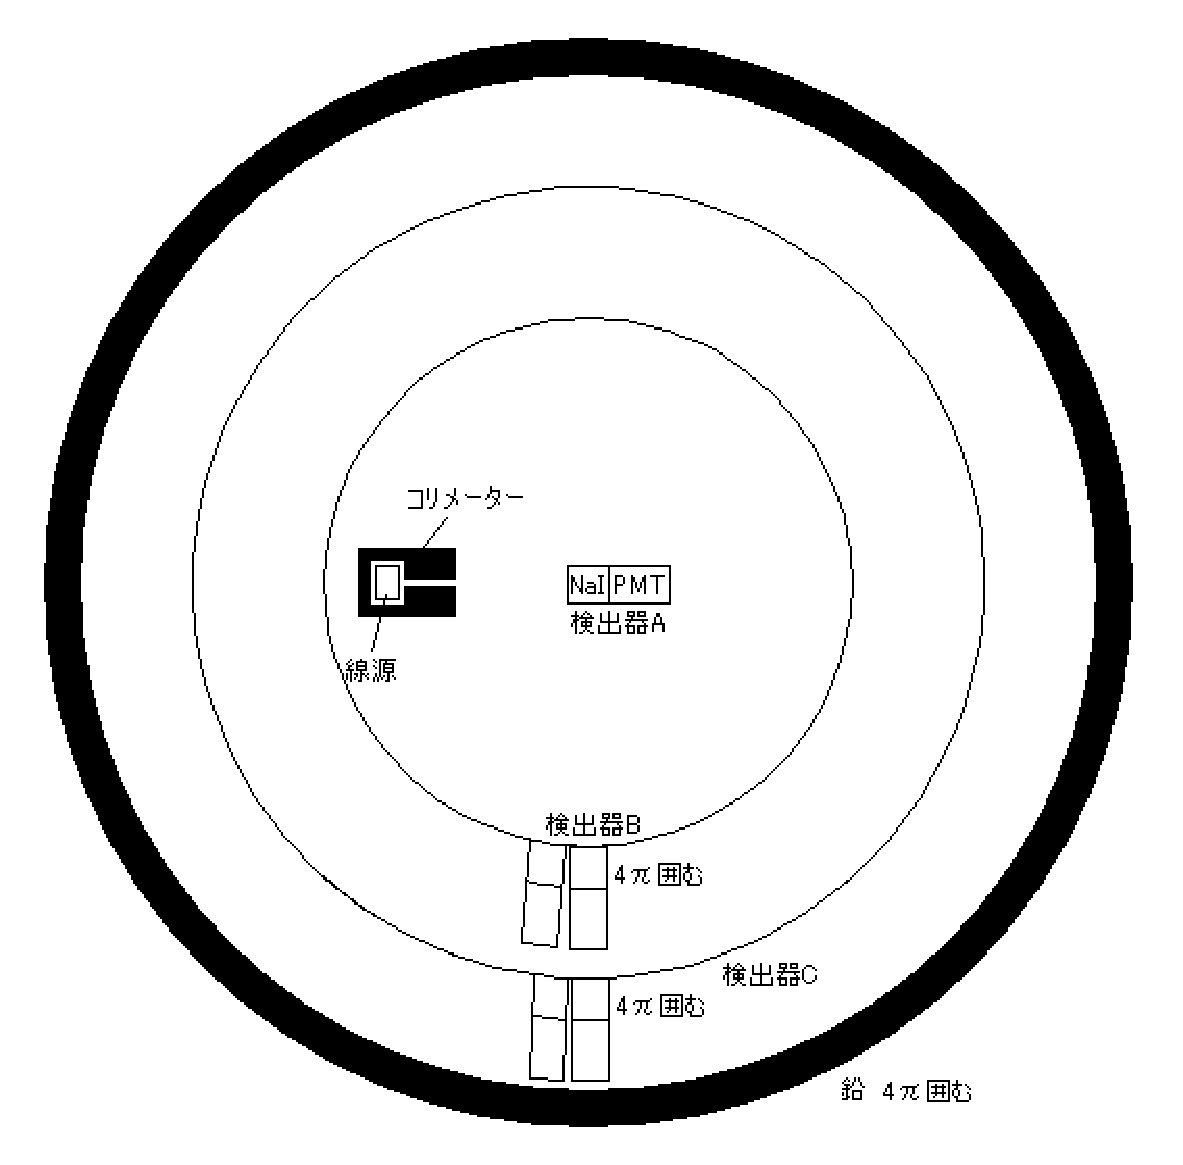
\includegraphics{2003phy5-9.eps}}
		\caption{(b)の実験装置の配置}
		\ilabel{5MeV setup}
  		\end{center}
\end{figure}

この場合は入射ガンマ線のエネルギーが大きいために断面積が、
\begin{eqnarray}
	コンプトン散乱>電子対生成 \gg 光電効果\simeq 0		\nonumber
\end{eqnarray}
となるので、問題の設定から、コンプトン散乱及び電子対生成による検出器Aにおける全エネルギーピークはほとんど得られないので、(a)で考えた方法は使えないことがわかる。これより、同じ検出器を使っていることから、同じ印加電圧を光電子増倍管にかけてやれば、増幅率も同じであり、同じエネルギーのガンマ線を入射させてやれば、得られる電流は同じである(当然2項分布の確率過程でありゆらぎは当然存在する)ということが仮定できる。つまり、(a)と同じように装置を組み立てるが、今度は検出器A及び検出器Bからの出力電流の全電流をまとめたものを考える。そうすると、検出器A及び検出器Bで全エネルギーを失う場合、これらを合計したものが全エネルギーとなり、全エネルギーを測定することができる。
このままだと検出器A及び検出器Bにおいて全エネルギーを失うイベントのみを拾うことが出来ずまたバックグラウンドが存在するので、検出器A及び線源と検出器Bの外側にさらに検出器で覆って、それを(a)での検出器Bのような逆計数にすることで、検出器A及び検出器Bで全エネルギーを失わなずにさらに外にエネルギーが漏れた場合のイベントを落とし、またバックグラウンドを含むイベントを除くことができる。この検出器のことを検出器Cと呼ぶことにする。本当はこの逆計数用にはプラスチックシンチレーターとかの方がよいと考えられる。そしてさらにその外側を、環境放射線が止まる程度の数cm程度の鉛などの遮蔽で(a)と同様に覆う。また、主なバックグラウンドである$\mu$粒子のStopping\ Powerが(a)で書いた通り$-\frac{ \mathrm{d} E}{\mathrm{d} x} \simeq 7 \ [\mathrm{MeV/cm}]$で表されるので、NaI(Tl)結晶の大きさは正確には書かれてはいないが、NaIシンチレーター中で$5 \ \mathrm{MeV}$前後という低いエネルギーを落とす確率は少なく、Discriminatorによって検出器A及び検出器Bのエネルギーのスレッショルドを、上限$6 \ \mathrm{MeV}$程度にしておくことでバックグラウンドによるイベントをより減らすことができると考えられる。さらに、同時計測におけるTimingを光速で走るところから計算して少し余裕を持たせて合わせるようにし、一イベント当たり検出器A及び検出器Bのうちエネルギーがその中で落とされた検出器の数があまりにも多いイベントや、一イベント当たりの電流を流した検出器に対し下限のスレッショルドもDiscriminatorで設けることでエネルギーの小さいものを除くことにより、全エネルギーを落としきれていないイベントやバックグラウンドの影響を除くことができると考えられる。最終的には全体として和が$5 \ \mathrm{MeV}$前後のところにくるピークを上下のスレッショルドをかけて残してやれば求めたい全エネルギーピークを見ることが出来る。(a)と同様に、(b)の装置もできたら真空槽に入れたほうがよい。
\end{enumerate}
\end{answer}


\end{document}
